\documentclass{article}
\usepackage[a4paper, margin=0.5in]{geometry}
\usepackage[utf8]{inputenc}
\usepackage{amsmath}
\usepackage{stmaryrd}
\usepackage{graphicx}
\usepackage{xcolor}

\renewcommand\t[1]{\text{#1}}
\renewcommand\d{\text{ . }}
\newcommand\lwt[1]{$_\text{#1}$}
\newcommand\TODO[1]{\textcolor{red}{TODO: #1}}

\usepackage{graphicx}

\begin{document}

% \maketitle

\section{}

\subsection*{a)}

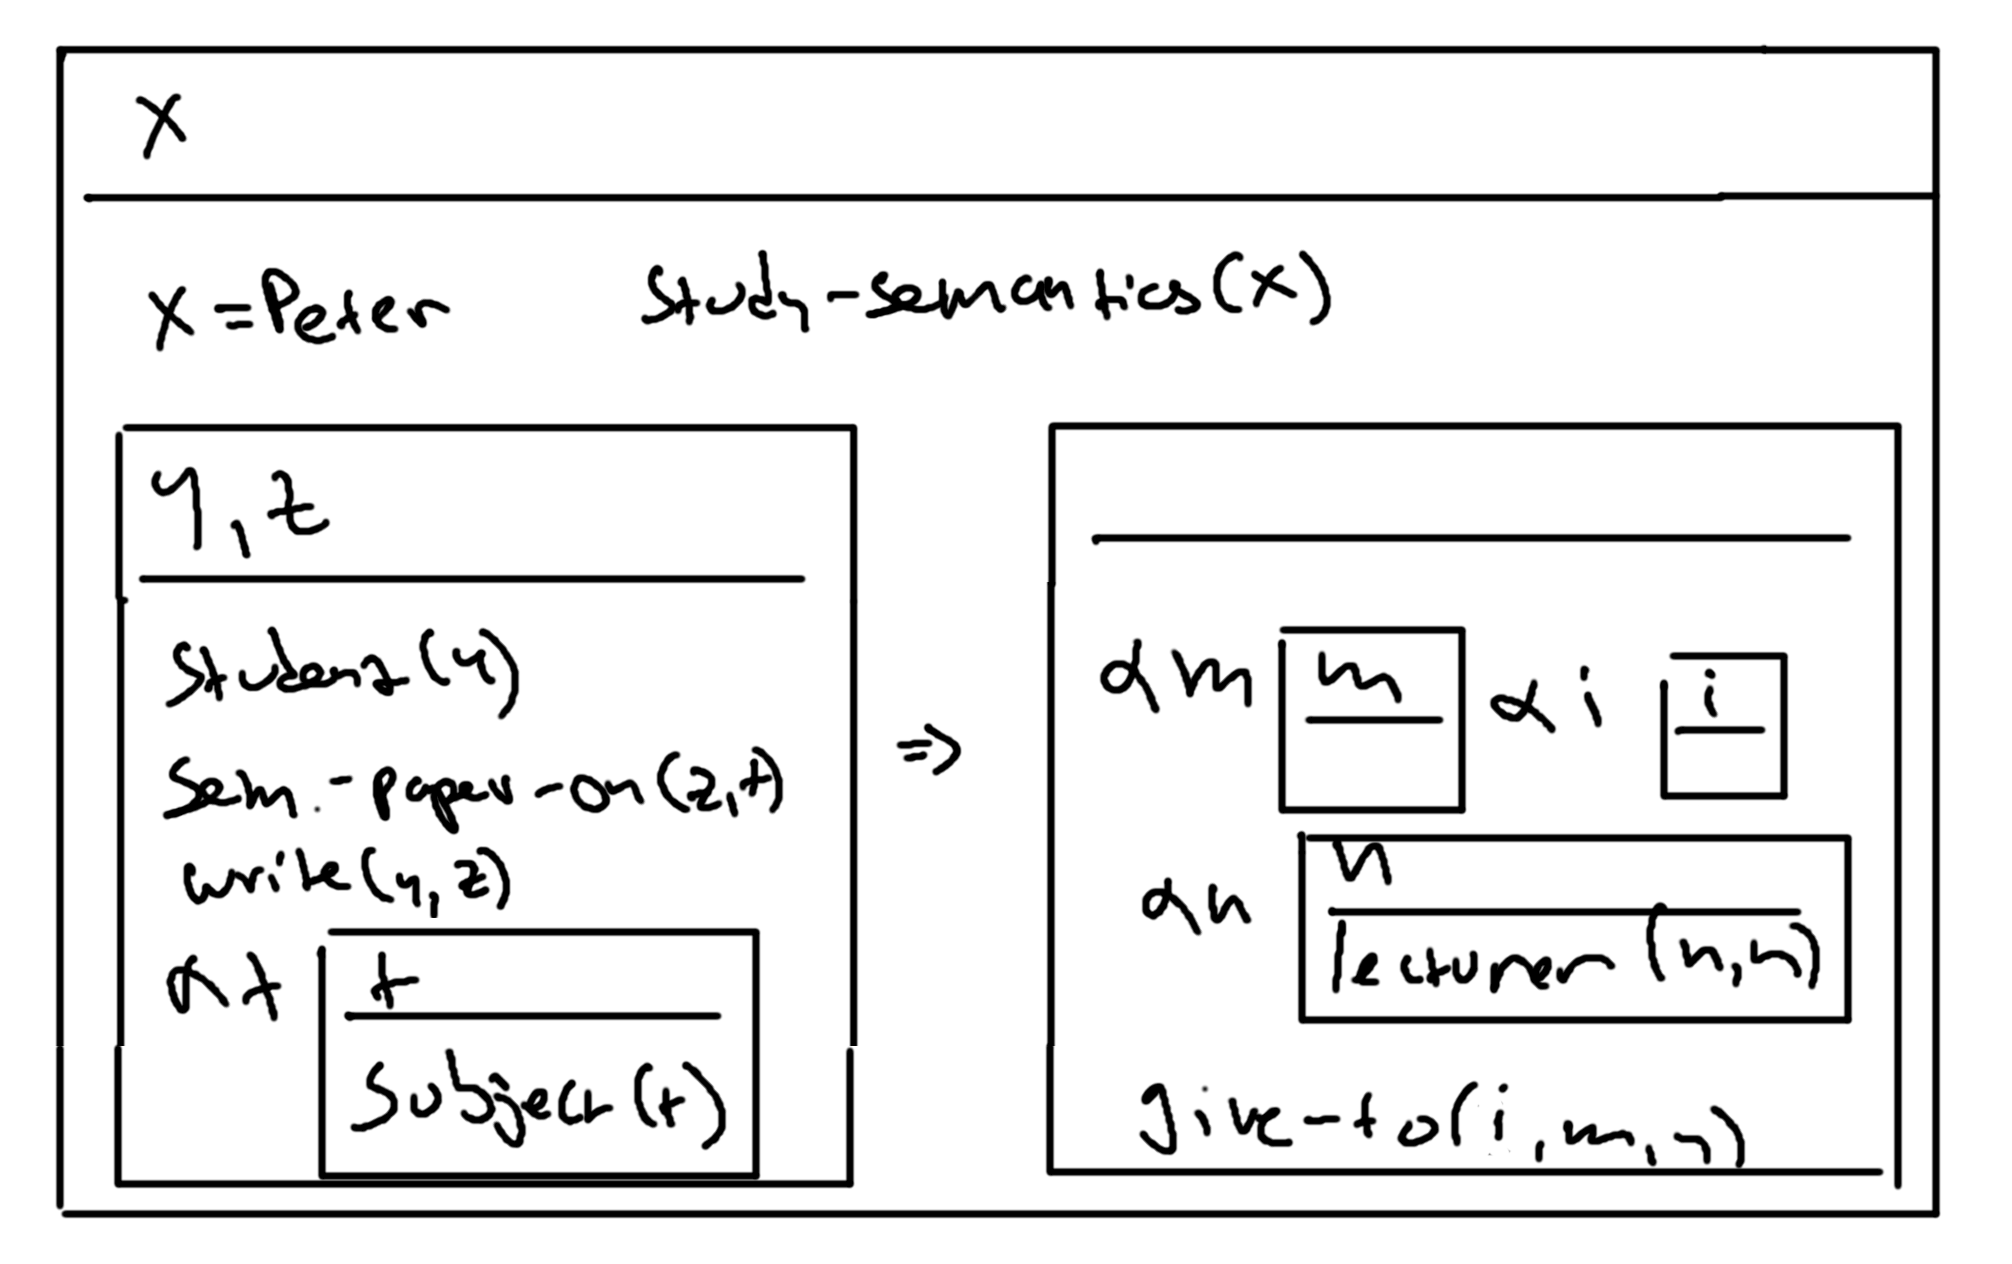
\includegraphics[width=0.75\linewidth]{drs_a.png}

\subsection*{b)}

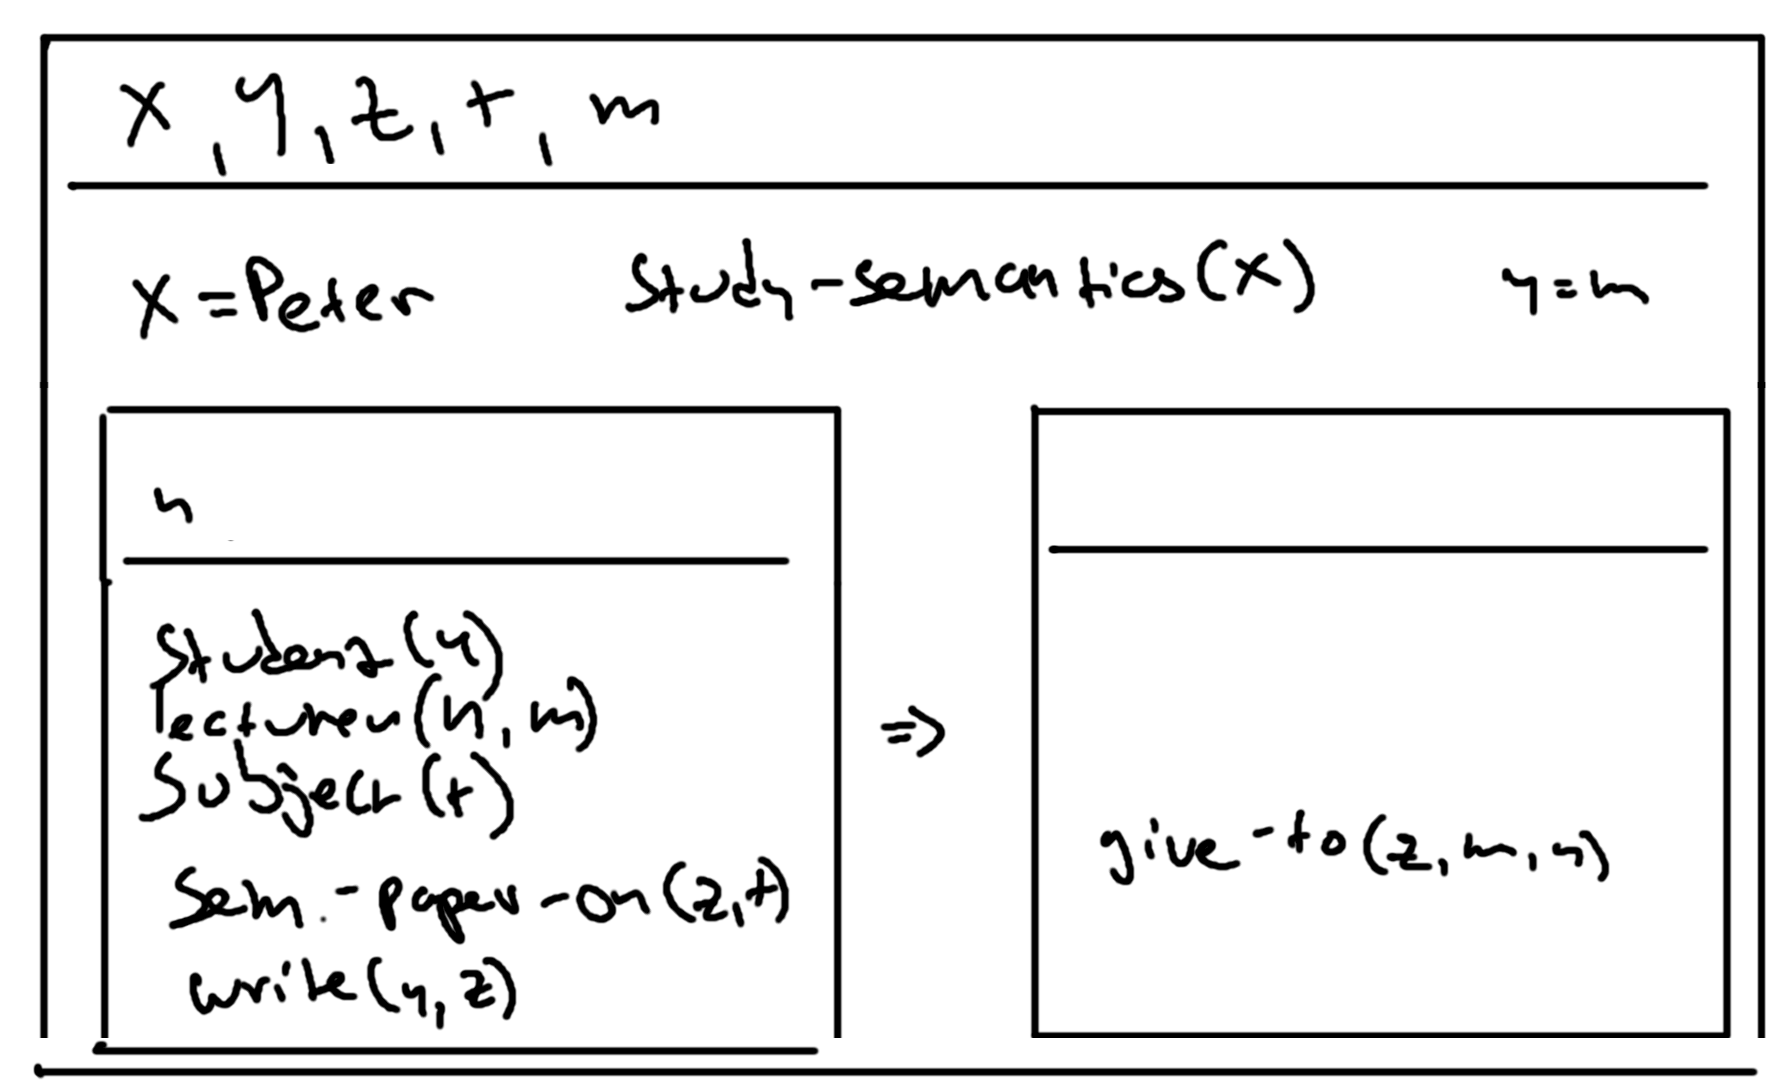
\includegraphics[width=0.75\linewidth]{drs_b.png}

The \emph{lecturer} was resolved via binding and the rest via accomodation.

\section{}

\subsection*{a)}

\begin{itemize}
\item[(2)] John owns a donkey
\item[(3)] -
\end{itemize}

There are also other, more subtle presupositions in both sentences, such as that donkeys can be owned, that they can eat and that they can potentially fit in the stable, that John is an existing entity which can own other entities and that stable is a thing in which entities can be.

\subsection*{b)}

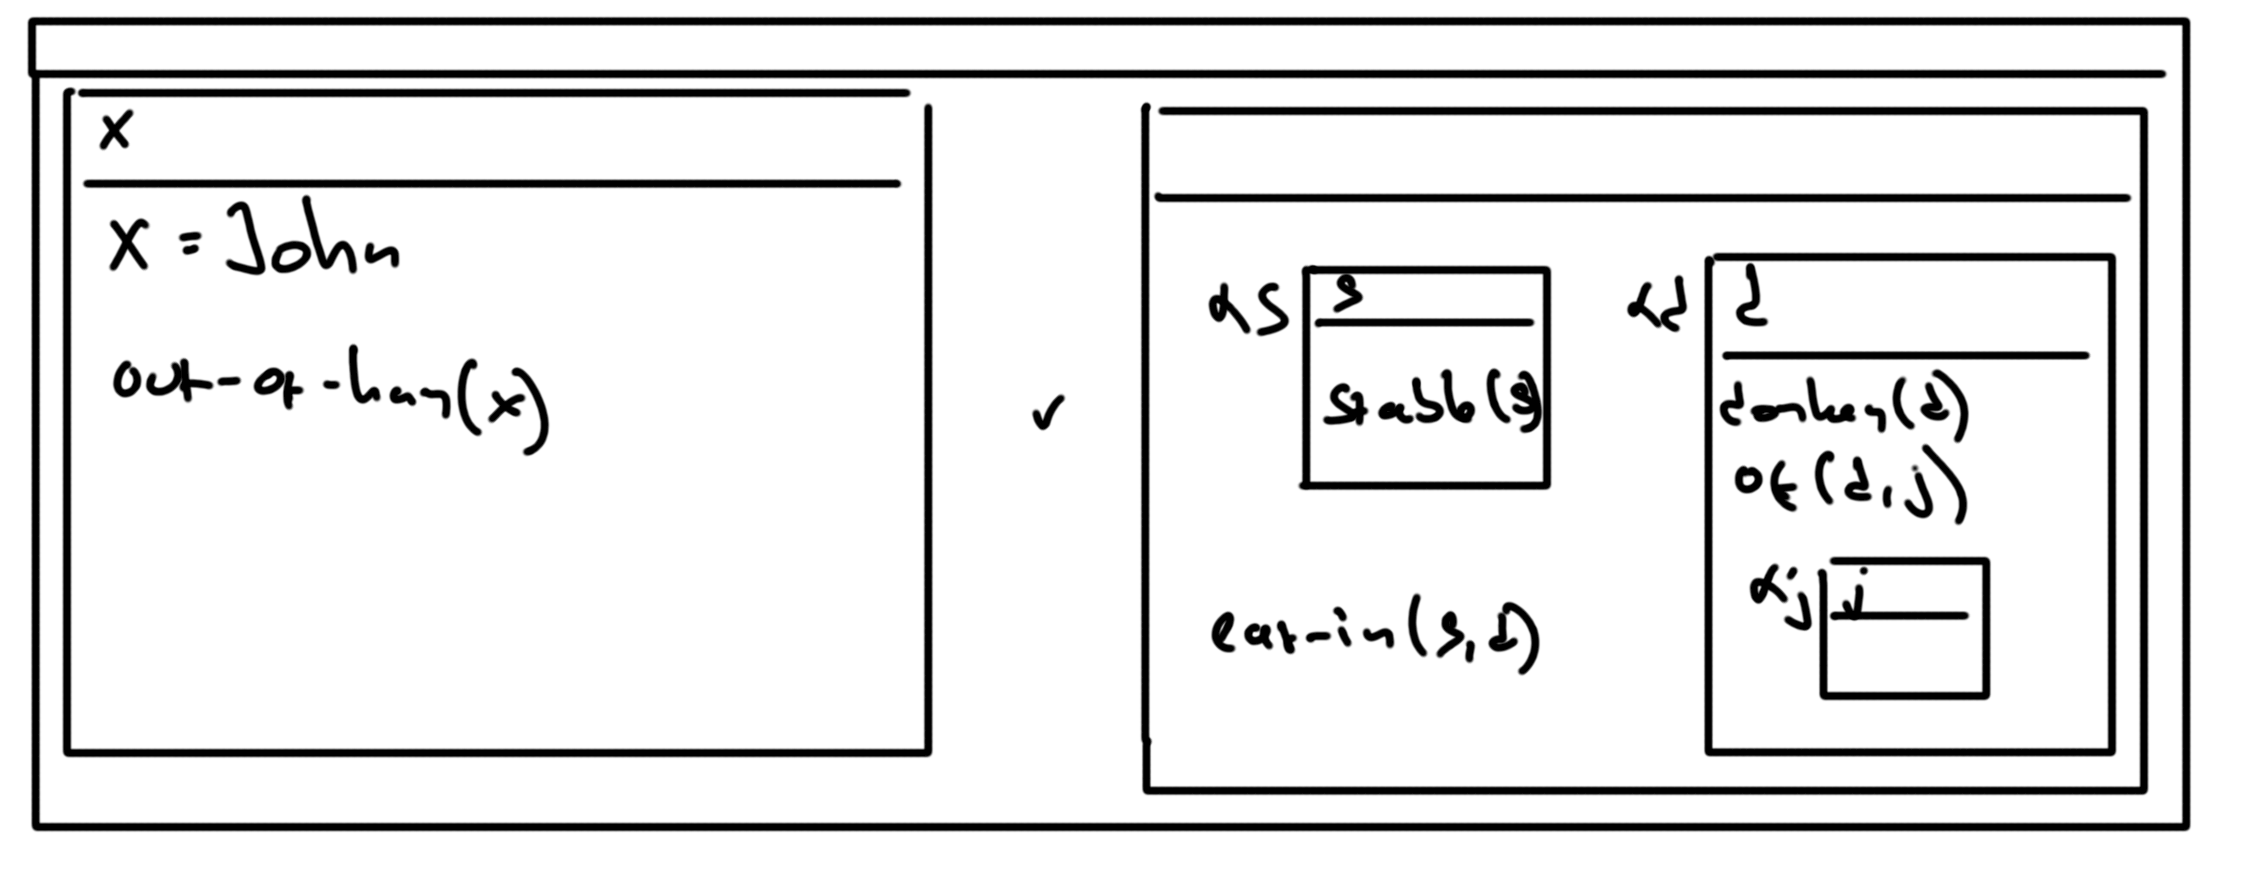
\includegraphics[width=0.75\linewidth]{dpr_2_a.png}

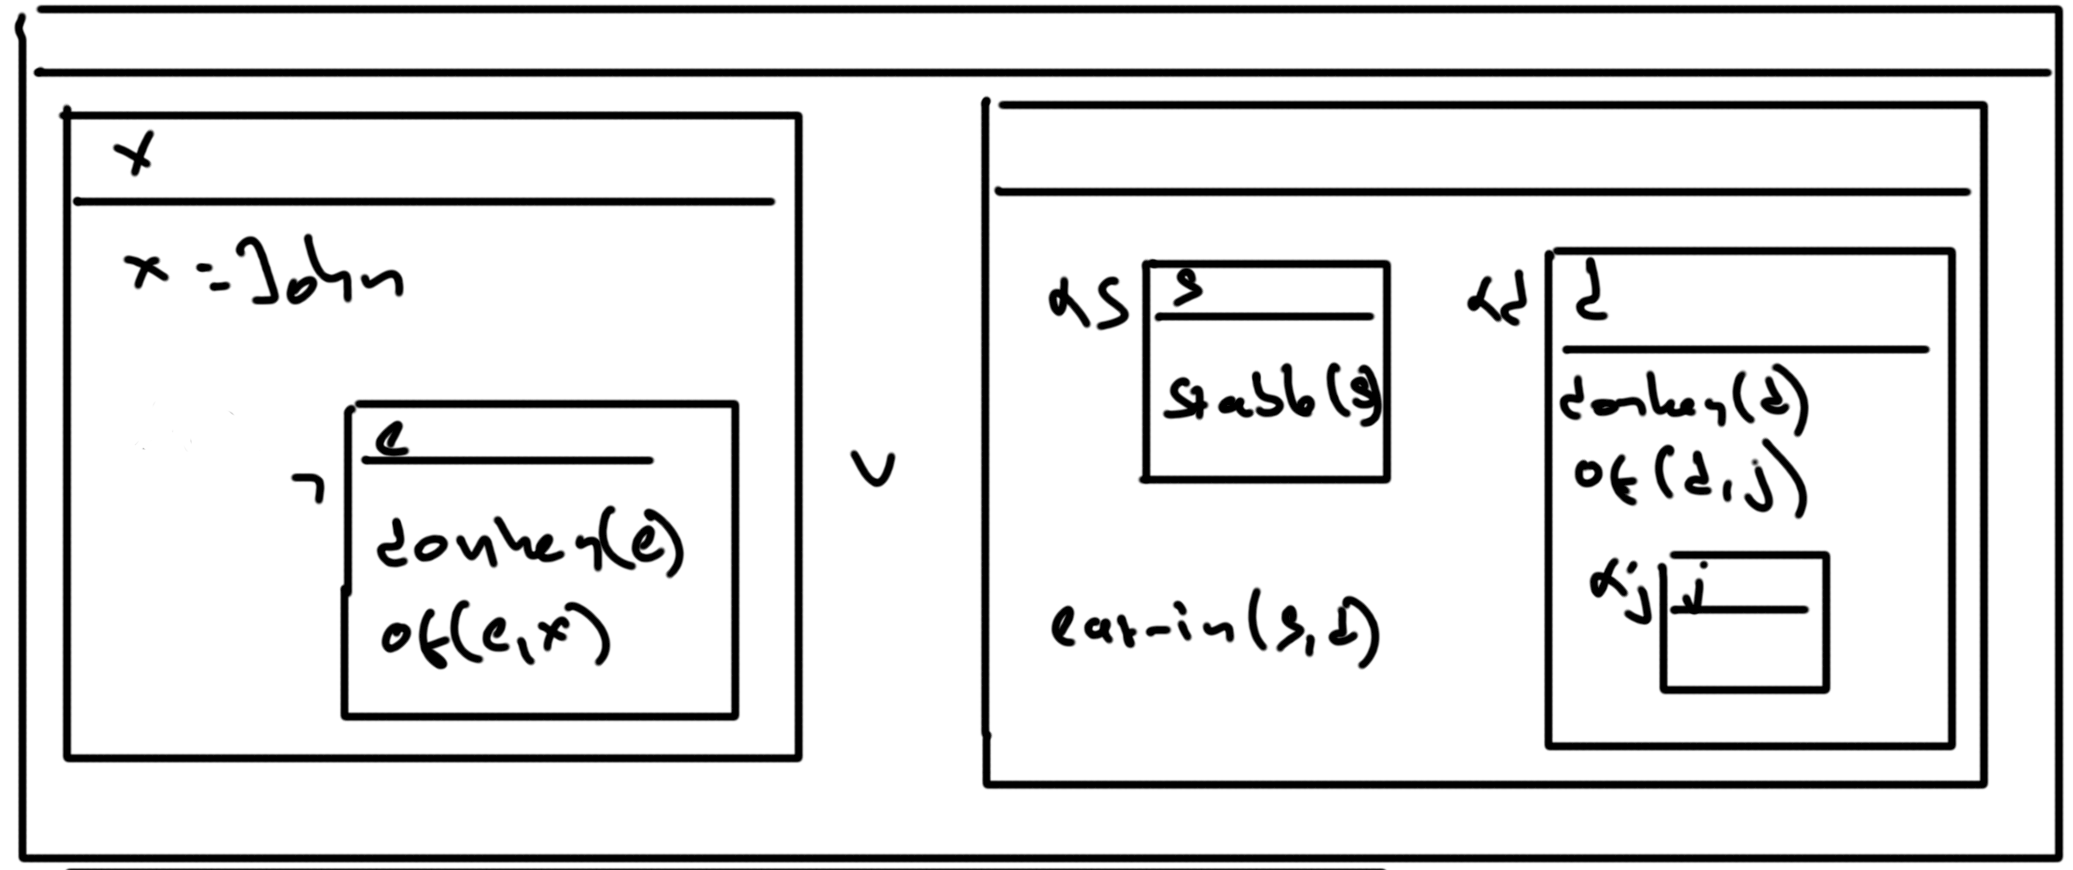
\includegraphics[width=0.75\linewidth]{dpr_3_a.png}

\subsection*{c)}

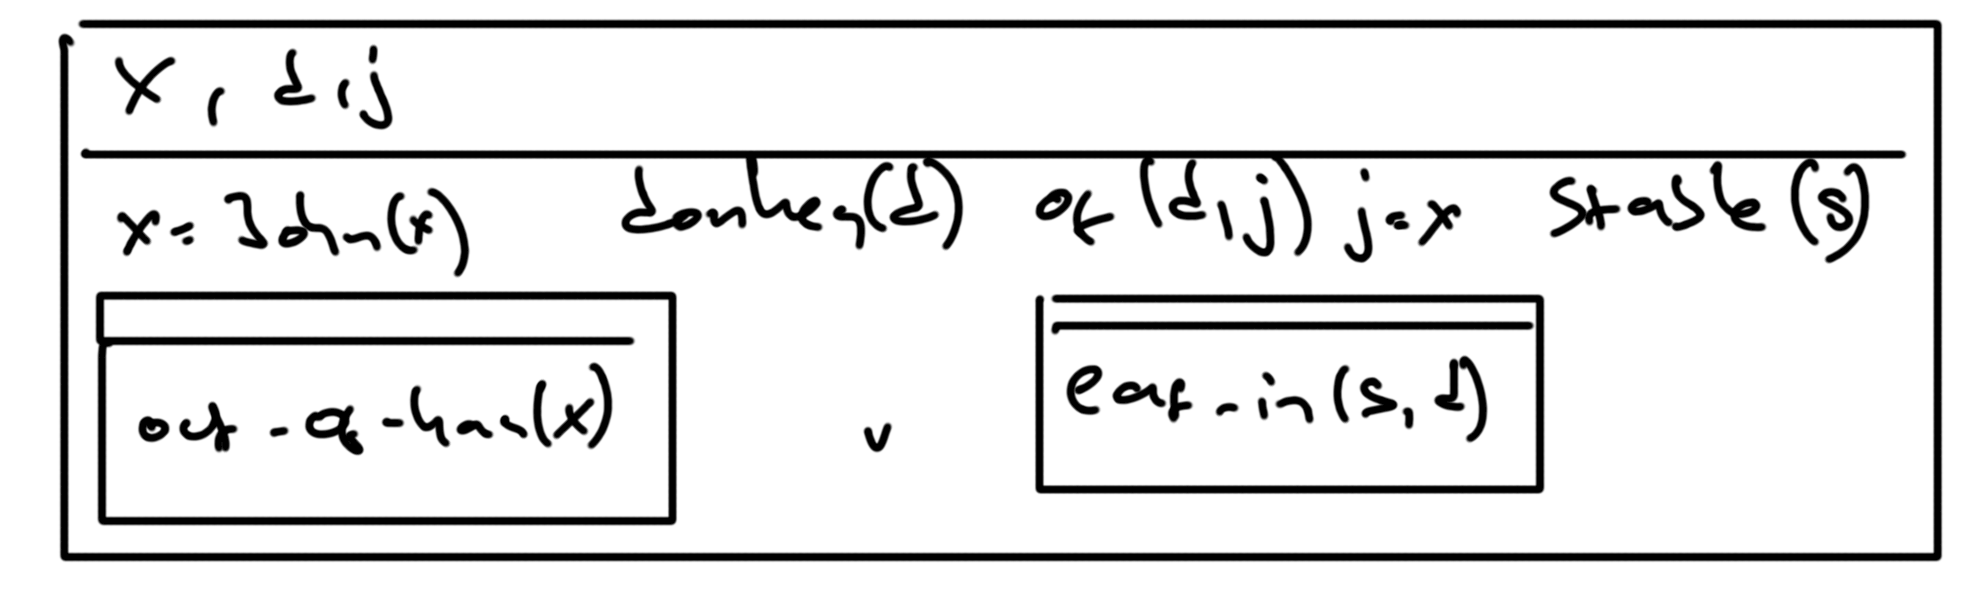
\includegraphics[width=0.75\linewidth]{dpr_2_b.png}

In the first case, everything was resolved using accomodation.

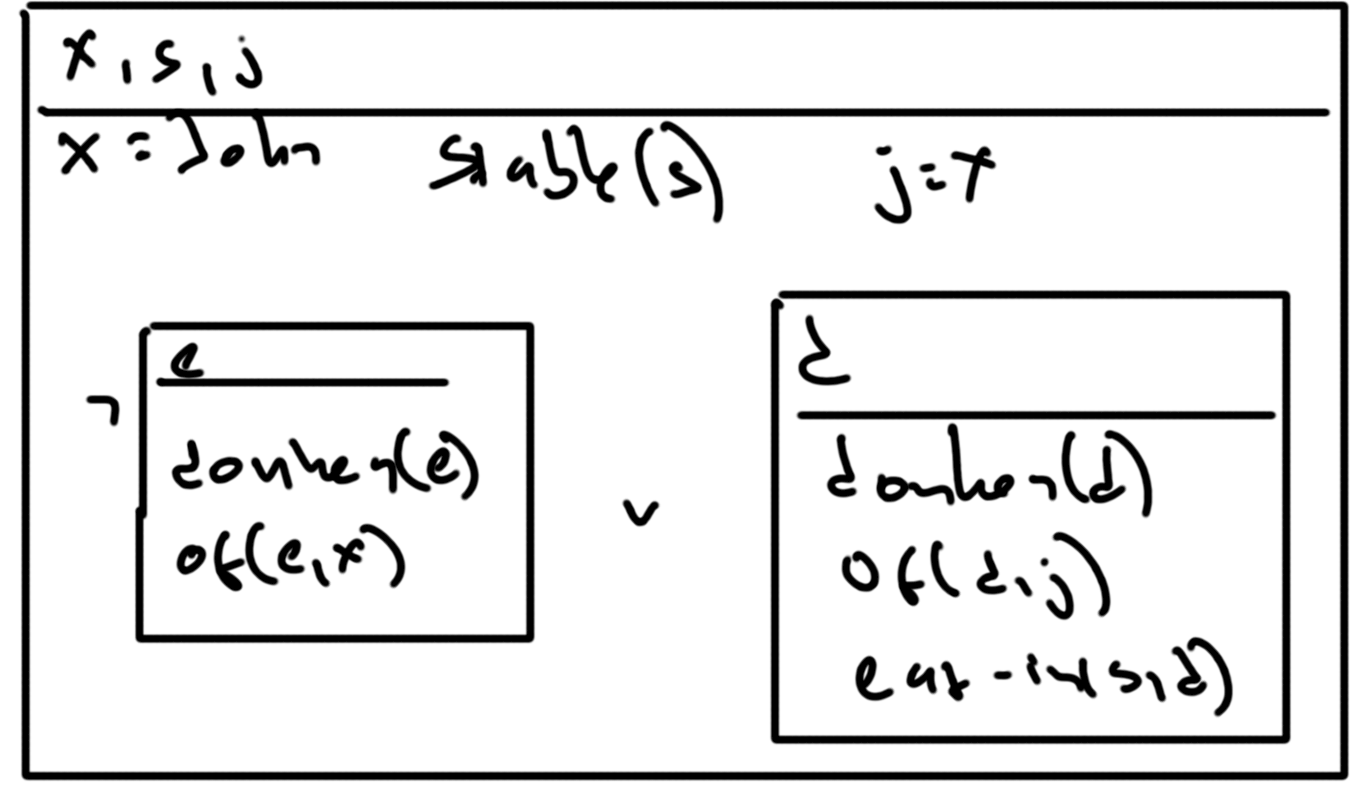
\includegraphics[width=0.75\linewidth]{dpr_3_b.png}

In the second case most of the things got shifted to the top-level DRS (accomodation) though the solution is probably not correct.

\end{document}
